\section{Аутентификация в веб-сервисах}
\selectlanguage{russian}

Протокол HTTP\index{протокол!HTTP} (вместе с HTTPS\index{протокол!HTTPS}) является, в настоящий момент, наиболее популярным протоколом, использующимся в сети Интернет для доступа к сервисам, таким как социальные сети или веб-клиенты электронной почты. Данный протокол является протоколом типа "запрос-ответ"\index{протокол!запрос-ответ}, причём для каждого запроса открывается новое соединение с сервером\footnote{Для версии протокола HTTP/1.0 существует неофициальное~\cite[p.~17]{Totty:2002} расширение в виде заголовка \texttt{Connection: Keep-Alive}, который позволяет использовать одно соединение для нескольких запросов. Версия протокола HTTP/1.1 по умолчанию~\cite[6.3.~Persistence]{rfc7230} устанавливает поддержку выполнения нескольких запросов в рамках одного соединения. Однако все запросы всё равно выполняются независимо друг от друга.}. То есть протокол HTTP не является сессионным протоколом\index{протокол!сессионный}. В связи с этим задачу аутентификации на веб-сервисах можно различить на задачи первичной и вторичной аутентификации. \textit{Первичной аутентификацией}\index{аутентификация!первичная} будем называть механизм обычной аутентификации пользователя в рамках некоторого HTTP-запроса, а \textit{вторичной}\index{аутентификация!вторичная} (или \textit{повторной}\index{аутентификация!повторная}) -- некоторый механизм подтверждения в рамках последующих HTTP-запросов, что пользователь уже был \textit{ранее} аутентифицирован веб-сервисом в рамках первичной аутентификации.

Аутентификация в веб-сервисах также бывает \textit{односторонней}\index{аутентификация!односторонняя} (как со стороны клиента, так и со стороны сервиса) и \textit{взаимной}\index{аутентификация!взаимная}. Под аутентификацией веб-сервиса обычно понимается возможность сервиса доказать клиенту, что он является именно тем веб-сервисом, к которому хочет получить доступ пользователь, а не его мошеннической подменой, созданной злоумышленниками. Для аутентификации веб-сервисов используется механизм сертификатов открытых ключей\index{сертификат открытого ключа} протокола HTTPS\index{протокол!HTTPS} с использованием инфраструктуры открытых ключей\index{инфраструктура открытых ключей} (см. раздел~\ref{chapter-public-key-infrastructure}).

При использовании протокола HTTPS\index{протокол!HTTPS} и наличии соответствующей поддержки со стороны веб-сервиса клиент также имеет возможность аутентифицировать себя с помощью своего сертификата открытого ключа\index{сертификат открытого ключа}. Данный механизм редко используется в публичных веб-сервисах, так как требует от клиента иметь на устройстве, с которого осуществляется доступ, файл сертификата открытого ключа.

\subsection{Первичная аутентификация по паролю}

Стандартная первичная аутентификация в современных веб-сервисах происходит обычной передачей логина и пароля в открытом виде по сети. Если SSL-соединение не используется, логин и пароль могут быть перехвачены. Даже при использовании SSL-соединения веб-приложение имеет доступ к паролю в открытом виде.

Более защищённым, но мало используемым способом аутентификации является вычисление хэша от пароля $m$, <<соли>> $s$ и псевдослучайных одноразовых меток $n_1, n_2$ с помощью JavaScript в браузере и отсылка по сети только результата вычисления хэша.
\[ \begin{array}{ll}
    \text{Браузер} ~\rightarrow~ \text{Сервис:} & \text{HTTP GET-запрос} \\
    \text{Браузер} ~\leftarrow~ \text{Сервис:}  & s ~\|~ n_1 \\
    \text{Браузер} ~\rightarrow~ \text{Сервис:} & n_2 ~\|~ h( h(s ~\|~ m) ~\|~ n_1 ~\|~ n_2) \\
\end{array} \]

Если веб-приложение хранит хэш от пароля и соли $h(s ~\|~ m)$, то пароль не может быть перехвачен ни по сети, ни веб-приложением.

В массовых интернет-сервисах пароли часто хранятся в открытом виде на сервере, что не является хорошей практикой для обеспечения защиты персональных данных пользователей.

\subsection{Первичная аутентификация в OpenID}
\selectlanguage{russian}

Из-за большого числа различных логинов, которые приходится использовать для доступа к разным сервисам, постепенно происходит внедрение единых систем аутентификации для разных сервисов (single sign-on), например, OpenID. Одновременно происходит концентрация пользователей вокруг больших порталов с единой аутентификацией, например, Google Account. Яндекс.Паспорт также уменьшает число используемых паролей для разных служб.

Принцип аутентификации состоит в следующем.
\begin{enumerate}
    \item Пользователи и интернет-сервисы доверяют аутентификацию третьей стороне -- центру единой аутентификации.
    \item Когда пользователь заходит на интернет-ресурс, веб-приложение перенаправляет его на центр аутентификации с защитой TLS-соединением.
    \item Центр аутентифицирует пользователя и выдает ему токен аутентификации, который пользователь предъявляет интернет-сервису.
    \item Сервис по токену аутентификации определяет имя пользователя.
\end{enumerate}

\begin{figure}[!ht]
	\centering
	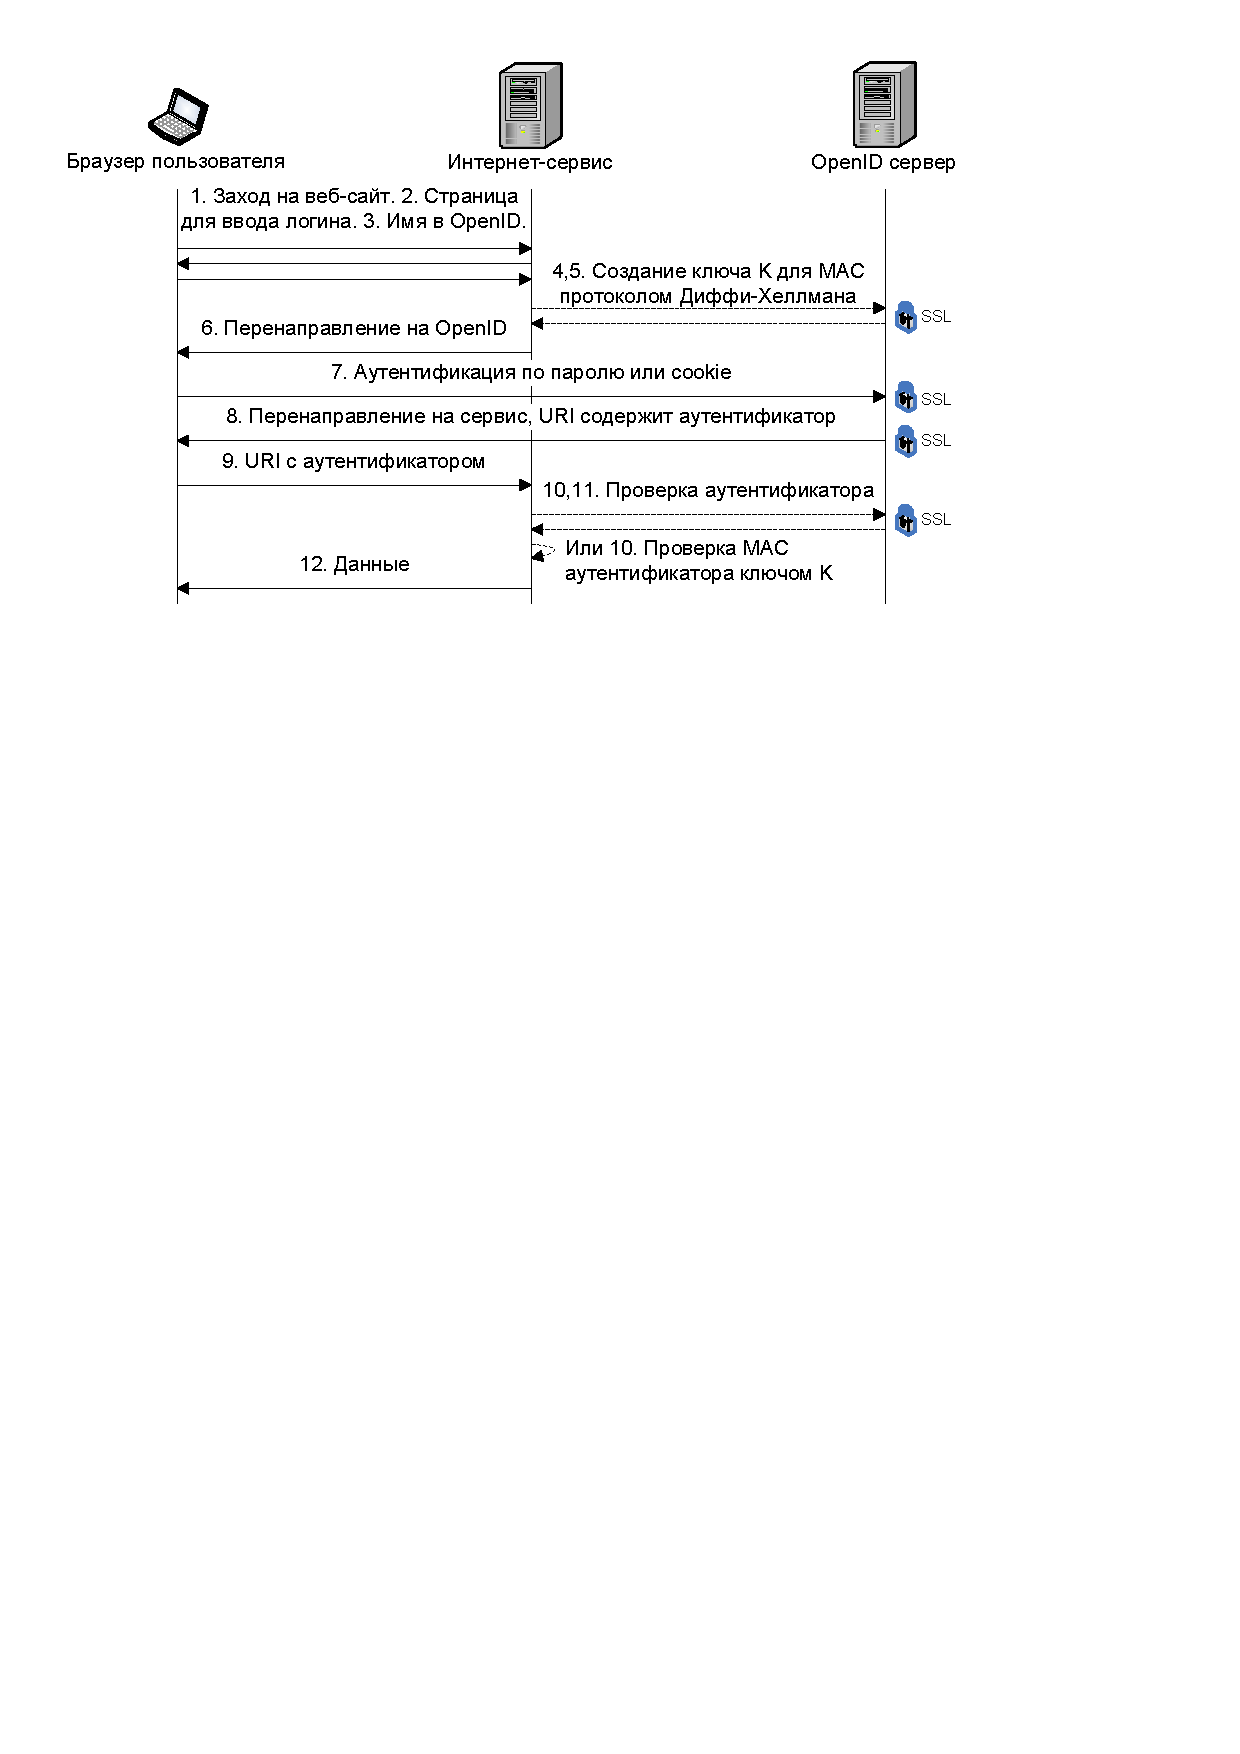
\includegraphics[width=0.9\textwidth]{pic/openid}
	\caption{Схема аутентификации в OpenID\label{fig:openid}}
\end{figure}

На рис.~\ref{fig:openid} показана схема аутентификации в OpenID версии 2 для доступа к стороннему интернет-сервису.

Если сервис и центр вместе создают общий секретный ключ $K$ для имитовставки\index{имитовставка} $\MAC_K$, выполняются шаги 4, 5 по протоколу Диффи~---~Хеллмана\index{протокол!Диффи~---~Хеллмана}:
\[ \begin{array}{l}
    \text{4. Сервис} ~\rightarrow~ \text{центр: модуль}~ p ~\text{группы}~ \Z_p^*, ~\text{генератор}~ g, \\
        ~~~~~~~~~~~~~~~\text{число}~ g^a \mod p, \\
    \text{5. Сервис} ~\leftarrow~ \text{центр: число}~ g^b \mod p, ~\text{гаммированный} \\
        ~~~~~~~~~~~~~~~\text{ключ}~ K \oplus (g^{ab} \mod p),
\end{array} \]
то аутентификатор содержит $\MAC_K$, проверяемый шагом 10, на выданном ключе $K$\footnote{Более правильным подходом является использование в качестве ключа $K = g^{ab} \mod p$, так как в этом случае ключ создается совместно, а не выдается центром.}. Имитовставка\index{имитовставка} определяется как описанный ранее $\HMAC$ с хэш-функцией SHA-256.

Если сервис и центр не создают общий ключ (этапы 4, 5 не выполняются), то сервис делает запрос на проверку аутентификатора в шагах 10, 11.

В OpenID аутентификатор состоит из следующих основных полей: имени пользователя, URL сервиса, результата аутентификации в OpenID, одноразовой метки и, возможно, кода аутентификации от полей аутентифкатора на секретном ключе $K$, если он был создан на этапах 4, 5. Одноразовая метка является \emph{одноразовым} псевдослучайным идентификатором результата аутентификации, который центр сохраняет в своей БД. По одноразовой метке сервис запрашивает центр о верности результата аутентификации на этапах 10, 11. Одноразовая метка дополнительно защищает от атак воспроизведения.

Можно было бы исключить шаги 4, 5, 10, 11, но тогда сервису бы пришлось реализовывать и хранить в БД использованные одноразовые метки для защиты от атак воспроизведения. Цель OpenID -- предоставить аутентификацию с минимальными издержками на интеграцию. Поэтому в OpenID реализуется модель, в которой сервис все проверки делегирует запросами к центру.

Важно отметить, что в аутентификации через OpenID необходимо использовать TLS-соединения\index{протокол!SSL/TLS} (то есть протокол HTTPS\index{протокол!HTTPS}) на всех взаимодействиях с центром, так как в самом протоколе OpenID не производится аутентификация сервиса и центра, конфиденциальность и целостность не поддерживаются.


\subsection{Вторичная аутентификация по cookie}
\selectlanguage{russian}

Протокол HTTP не поддерживает запоминание состояния соединения. Все запросы браузера интернет-сервису неотличимы от того, происходят они в первый раз или последующие. Поэтому для образования связности взаимодействия браузера и интернет-сервиса вводят искусственно <<состояние>> либо с помощью cookie, либо внедряют как часть URL, либо применяя скрытые элементы в формах.

Пример передачи переменных через URL: \\
\texttt{http://en.wikipedia.org/w/index.php? \\
\hspace*{1 cm} title=Hypertext\_Transfer\_Protocol\& \\
\hspace*{1 cm} action=historysubmit\&diff=330577492\&oldid=330543455}, \\
где браузер при запросе к веб-сервису указывает значения переменных: \texttt{ \\
\hspace*{1 cm} title = Hypertext\_Transfer\_Protocol, \\
\hspace*{1 cm} action = historysubmit, \\
\hspace*{1 cm} diff = 330577492, \\
\hspace*{1 cm} oldid = 330543455.
}

В скрытых элементах форм языка разметки HTML, которые не показываются браузером на веб-странице, веб-сервер передает установленные значения переменных, которые браузер отправит назад сервису вместе с отправкой других видимых полей формы: \texttt{ \\
\hspace*{1 cm} <input type="hidden"\ name="user"\ value="john"/> \\
\hspace*{1 cm} <input type="hidden"\ name="birthdate" \\
\hspace*{2 cm}      value="29.02.1986"/> \\
\hspace*{1 cm} <input type="hidden"\ name="age"\ value="3"/>
}

Вторичная аутентификация при каждом HTTP-запросе, как правило, реализуется через cookie, которые браузер сохраняет в своем кэше посещенных страниц. Первоначально cookie были разработаны для возможности создания интернет-магазина.

Когда браузер в первый раз делает HTTP-запрос
\begin{center} \begin{verbatim}
GET /index.html HTTP/1.1
Host: www.wikipedia.org
\end{verbatim} \end{center}
к веб-серверу, веб-приложение сервера может отправить HTTP-пакет, содержащий параметр, строку текста, cookie:
\begin{center} \begin{verbatim}
HTTP/1.1 200 OK
Content-type: text/html
Set-Cookie: name1=value1; name2=value2; ...

...далее HTML-страница...
\end{verbatim} \end{center}
Браузер при последующих запросах к веб-серверу автоматически будет отсылать cookie назад веб-приложению
\begin{center} \begin{verbatim}
GET /wiki/HTTP_cookie HTTP/1.1
Host: www.wikipedia.org
Cookie: name1=value1; name2=value2; ...
Accept: */*
\end{verbatim} \end{center}

Далее веб-приложение может создать новый cookie и т.д. Браузер хранит cookie на диске в кэш-памяти. То есть cookie -- это возможность хранить переменные локально в кэш-памяти браузера, отсылать сохраненные значения, получать новые переменные. Фактически cookie дают возможность <<продолжать>> работу с интернет-сервисом с прежнего момента после закрытия и открытия браузера, а не заново.

В результате создается передача состояний, что дает возможность не вводить логин и пароль каждый раз при входе в интернет-сервис, использовать несколько окон для одного сеанса работы в интернет-магазине и т.д. При создании cookie может указываться его конечное время действия, после которого браузер удалит устаревший cookie.

Для вторичной аутентификации в cookie веб-приложение записывает аутентификатор в виде текстовой строки.

В качестве аутентификатора можно использовать \emph{псевдослучайную} текстовую строку достаточной длины, сгенерированную веб-приложением. Веб-приложение должно вести журнал выданных аутентификаторов пользователям и их сроков действия. Например,
\begin{center} \begin{verbatim}
Cookie: auth=B35NMVNASUY26MMWNVZ87
\end{verbatim} \end{center}

Вторым способом аутентификации является применение кода аутентификации сообщений ко всем данным, записанным в cookie. Код аутентификации сообщений $\MAC_K$ на секретном ключе $K = h(m \| s)$, который является хэшем от пароля $m$ и соли $s$, вычисляется от псевдослучайной одноразовой метки $\textrm{nonce}$, имени пользователя $user$ и других данных $data$, сохраняемых в cookie:
\begin{center} \begin{verbatim}
Cookie: User=user; Nonce=nonce; Data=data; MAC=auth;
\end{verbatim} \end{center}
    \[ auth = \HMAC_K(user \| \textrm{nonce} \| data). \]

Псевдослучайный аутентификатор предпочтительнее, так как позволяет гарантировать, что аутентификатор был создан веб-приложением, и не раскрывает имени пользователя. Использование кода аутентификации сообщения является дополнительной мерой того, что данные, сохраняемые в cookie, не были подделаны.

Конечно, беспокоиться об аутентификации в интернет-сервисах при использовании обычного HTTP-протокола без зашифрованного SSL-соединения имеет смысл только по отношению к угадыванию токенов аутентификации другими пользователями, которые не имеют доступа к маршрутизаторам и сети, через которые общается пользователь. Кража компьютера или одного cookie-файла, перехват незащищенного трафика HTTP-протокола приводят к доступу в систему под именем взломанного пользователя.

